\documentclass[dvipsnames,tikz]{standalone}
\usepackage{amsmath}
\usepackage{xcolor}
\usepackage{tikz}
\usetikzlibrary{calc}
\usetikzlibrary{decorations.pathreplacing,calligraphy,3d}


\begin{document}
	% add color=white for dark mode
	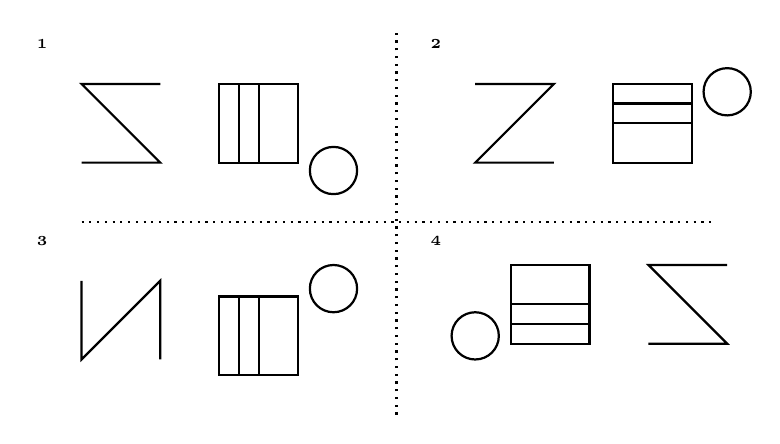
\begin{tikzpicture}[node distance={15mm}, thick, main/.style = {draw}] 
		\draw[dotted] (0,-0.75) -- (8,-0.75);
		\draw[dotted] (4,-3.2) -- (4,1.7);
		\begin{scope}
			\draw[font=\tiny] (-0.5,1.5) node {$\mathbf{1}$};
			\begin{scope}
				\path[shape=coordinate]	
				(1,0) coordinate(A) 
				(0,0) coordinate(B) 
				(1,1) coordinate(C) 
				(0,1) coordinate(D);
				
				\draw (B) -- (A) -- (D) -- (C);
			\end{scope}
			
			\begin{scope}[xshift=1.75cm, rotate around={90:(0.5,0.5)}]
				\path[shape=coordinate]	
				(0,0) coordinate(A) 
				(1,0) coordinate(B) 
				(1,1) coordinate(C) 
				(0,1) coordinate(D)
				(1,0.5) coordinate(E)
				(0,0.5) coordinate(F)
				(1,0.75) coordinate(G)
				(0,0.75) coordinate(H);
				
				\draw (A) -- (B) -- (C) -- (D) --cycle;
				\draw (E) -- (F);
				\draw (G) -- (H);
			\end{scope}
			
			\begin{scope}[xshift=3.2cm]
				\draw (0,-0.1) circle (0.3);
			\end{scope}
		\end{scope}
		
		\begin{scope}[xshift=5cm]
			\draw[font=\tiny] (-0.5,1.5) node {$\mathbf{2}$};
			\begin{scope}
				\path[shape=coordinate]	
				(1,0) coordinate(A) 
				(0,0) coordinate(B) 
				(1,1) coordinate(C) 
				(0,1) coordinate(D);
				
				\draw (A) -- (B) -- (C) -- (D);
			\end{scope}
			
			\begin{scope}[xshift=1.75cm]
				\path[shape=coordinate]	
				(0,0) coordinate(A) 
				(1,0) coordinate(B) 
				(1,1) coordinate(C) 
				(0,1) coordinate(D)
				(1,0.5) coordinate(E)
				(0,0.5) coordinate(F)
				(1,0.75) coordinate(G)
				(0,0.75) coordinate(H);
				
				\draw (A) -- (B) -- (C) -- (D) --cycle;
				\draw (E) -- (F);
				\draw (G) -- (H);
			\end{scope}
			
			\begin{scope}[xshift=3.2cm]
				\draw (0,0.9) circle (0.3);
			\end{scope}
		\end{scope}
		
		\begin{scope}[yshift=-2.5cm]
			\draw[font=\tiny] (-0.5,1.5) node {$\mathbf{3}$};
			\begin{scope}
				\path[shape=coordinate]	
				(1,0) coordinate(A) 
				(0,0) coordinate(B) 
				(1,1) coordinate(C) 
				(0,1) coordinate(D);
				
				\draw (A) -- (C) -- (B) -- (D);
			\end{scope}
			
			\begin{scope}[xshift=1.75cm, yshift=-0.2cm, rotate around={90:(0.5,0.5)}]
				\path[shape=coordinate]	
				(0,0) coordinate(A) 
				(1,0) coordinate(B) 
				(1,1) coordinate(C) 
				(0,1) coordinate(D)
				(1,0.5) coordinate(E)
				(0,0.5) coordinate(F)
				(1,0.75) coordinate(G)
				(0,0.75) coordinate(H);
				
				\draw (A) -- (B) -- (C) -- (D) --cycle;
				\draw (E) -- (F);
				\draw (G) -- (H);
			\end{scope}
			
			\begin{scope}[xshift=3.2cm]
				\draw (0,0.9) circle (0.3);
			\end{scope}
		\end{scope}
		
		\begin{scope}[yshift=-2.5cm, xshift=5cm]
			\draw[font=\tiny] (-0.5,1.5) node {$\mathbf{4}$};
			\begin{scope}[rotate around={180:(1.6,0.6)}]
				\begin{scope}
					\path[shape=coordinate]	
					(1,0) coordinate(A) 
					(0,0) coordinate(B) 
					(1,1) coordinate(C) 
					(0,1) coordinate(D);
					
					\draw (B) -- (A) -- (D) -- (C);
				\end{scope}
				
				\begin{scope}[xshift=1.75cm]
					\path[shape=coordinate]	
					(0,0) coordinate(A) 
					(1,0) coordinate(B) 
					(1,1) coordinate(C) 
					(0,1) coordinate(D)
					(1,0.5) coordinate(E)
					(0,0.5) coordinate(F)
					(1,0.75) coordinate(G)
					(0,0.75) coordinate(H);
					
					\draw (A) -- (B) -- (C) -- (D) --cycle;
					\draw (E) -- (F);
					\draw (G) -- (H);
				\end{scope}
				
				\begin{scope}[xshift=3.2cm]
					\draw (0,0.9) circle (0.3);
				\end{scope}
			\end{scope}
		\end{scope}
	\end{tikzpicture} 
	
\end{document}